\subsubsubsection{non-native-mul}

\begin{enumerate}
    \item \verb|Target|: Check the multiplication relation among three non-native target objects.
    \item \verb|Constraints logic|:
    \begin{itemize}
        \item Check equation for gadget: \verb|a * b = prod + modular * overflow|;
        \item Check that ``overflow.limb is U32'';
        \item Check that ``prod.limb is U32''.
    \end{itemize}
    \item \verb|Process layout|: See \ref{fig:non-native-mul-layout}.
    \item \verb|Constraints info and costs|:
    \begin{itemize}
        \item gadget biguint-add num: 1
        \item gadget biguint-mul num: 2
        \item gadget u32rangecheck num: 2
        \item gate type num: 9 = 7 (U32AddManyGate\{3,5,7,9,11,13,15\}) + 1 (U32RangeCheckGate) + 1 (U32ArithmeticGate)
        \item gate instance num: 37 = 2 (u32rangecheck) + 8 (biguint-mul: constant-input) + 22 (biguint-mul) + 1 + 3 (biguint-add)
        \item copy-constraints: 583 = 8 * 2 (u32rangecheck) + 3 * 3 + (4 + 6 + 8 + 10 + 12 + 14 + 16) * 4 + (8 * 8) * 3 + 17 * 4 + 18
    \end{itemize}
\end{enumerate}

\begin{figure}[!ht]
    \centering
    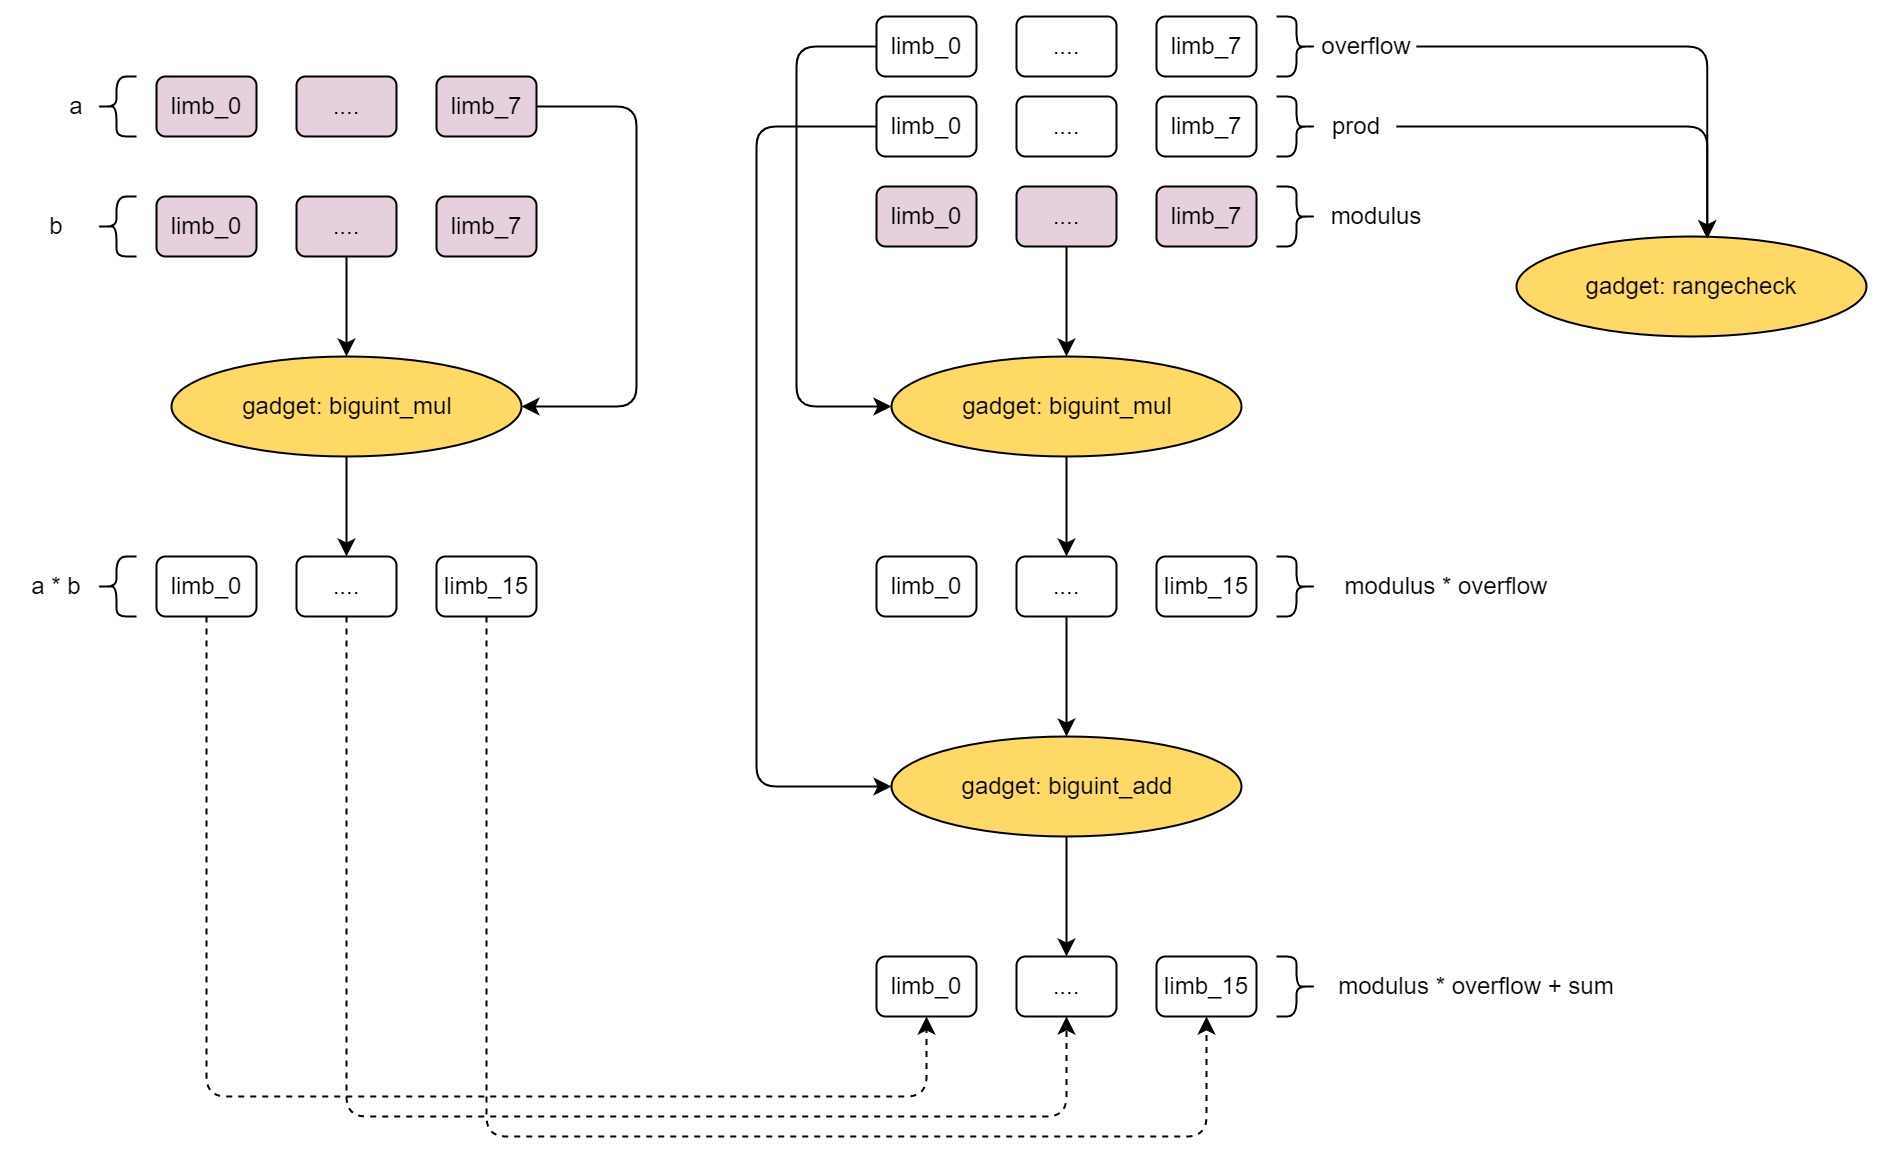
\includegraphics[width=0.6\textwidth]{nonnative-mul-layout.jpg}
    \caption{non-native-mul layout}
    \label{fig:non-native-mul-layout}
\end{figure}